\chapter{Results and discussion}
\label{Results-discussion-chapter}
In this work, we discuss potential \textit{more than Moore} applications of graphene-based devices through theoretical studies associated with experiments for real insights on the functionality of the sensory action of graphene. We emphasised the significance of humidity and carbon dioxide on graphene-based devices from a first-principle calculations point of view as well as the effect coming from the substrate. We also highlighted the possibility of passivating such sensors and making the device non-functional for serving the purpose of better integrity into \textit{more than Moore} applications.  

The results are presented in full in the attached seven manuscripts as in five published articles and two in the manuscript format under submission. Here, we provide a summary of these papers and how they connect.

To study graphene-based sensors theoretically, we carried out DFT calculations for examining and simulating the effect of the presence of adsorbates of carbon dioxide and water molecules on top of graphene. We constructed the supercells and set up the calculations in light of the calculational details discussed in Chapter \ref{chapter:calcDetails}. We calculated the binding distances, energies, charge transfer, charge density differences (CDD) and density of states for supercells of pristine graphene with adsorbates on top while the substrate is intact. We took care of the dispersive forces as reviewed in Chapter \ref{DFT-chapter}. 

\begin{figure}
    \centering
    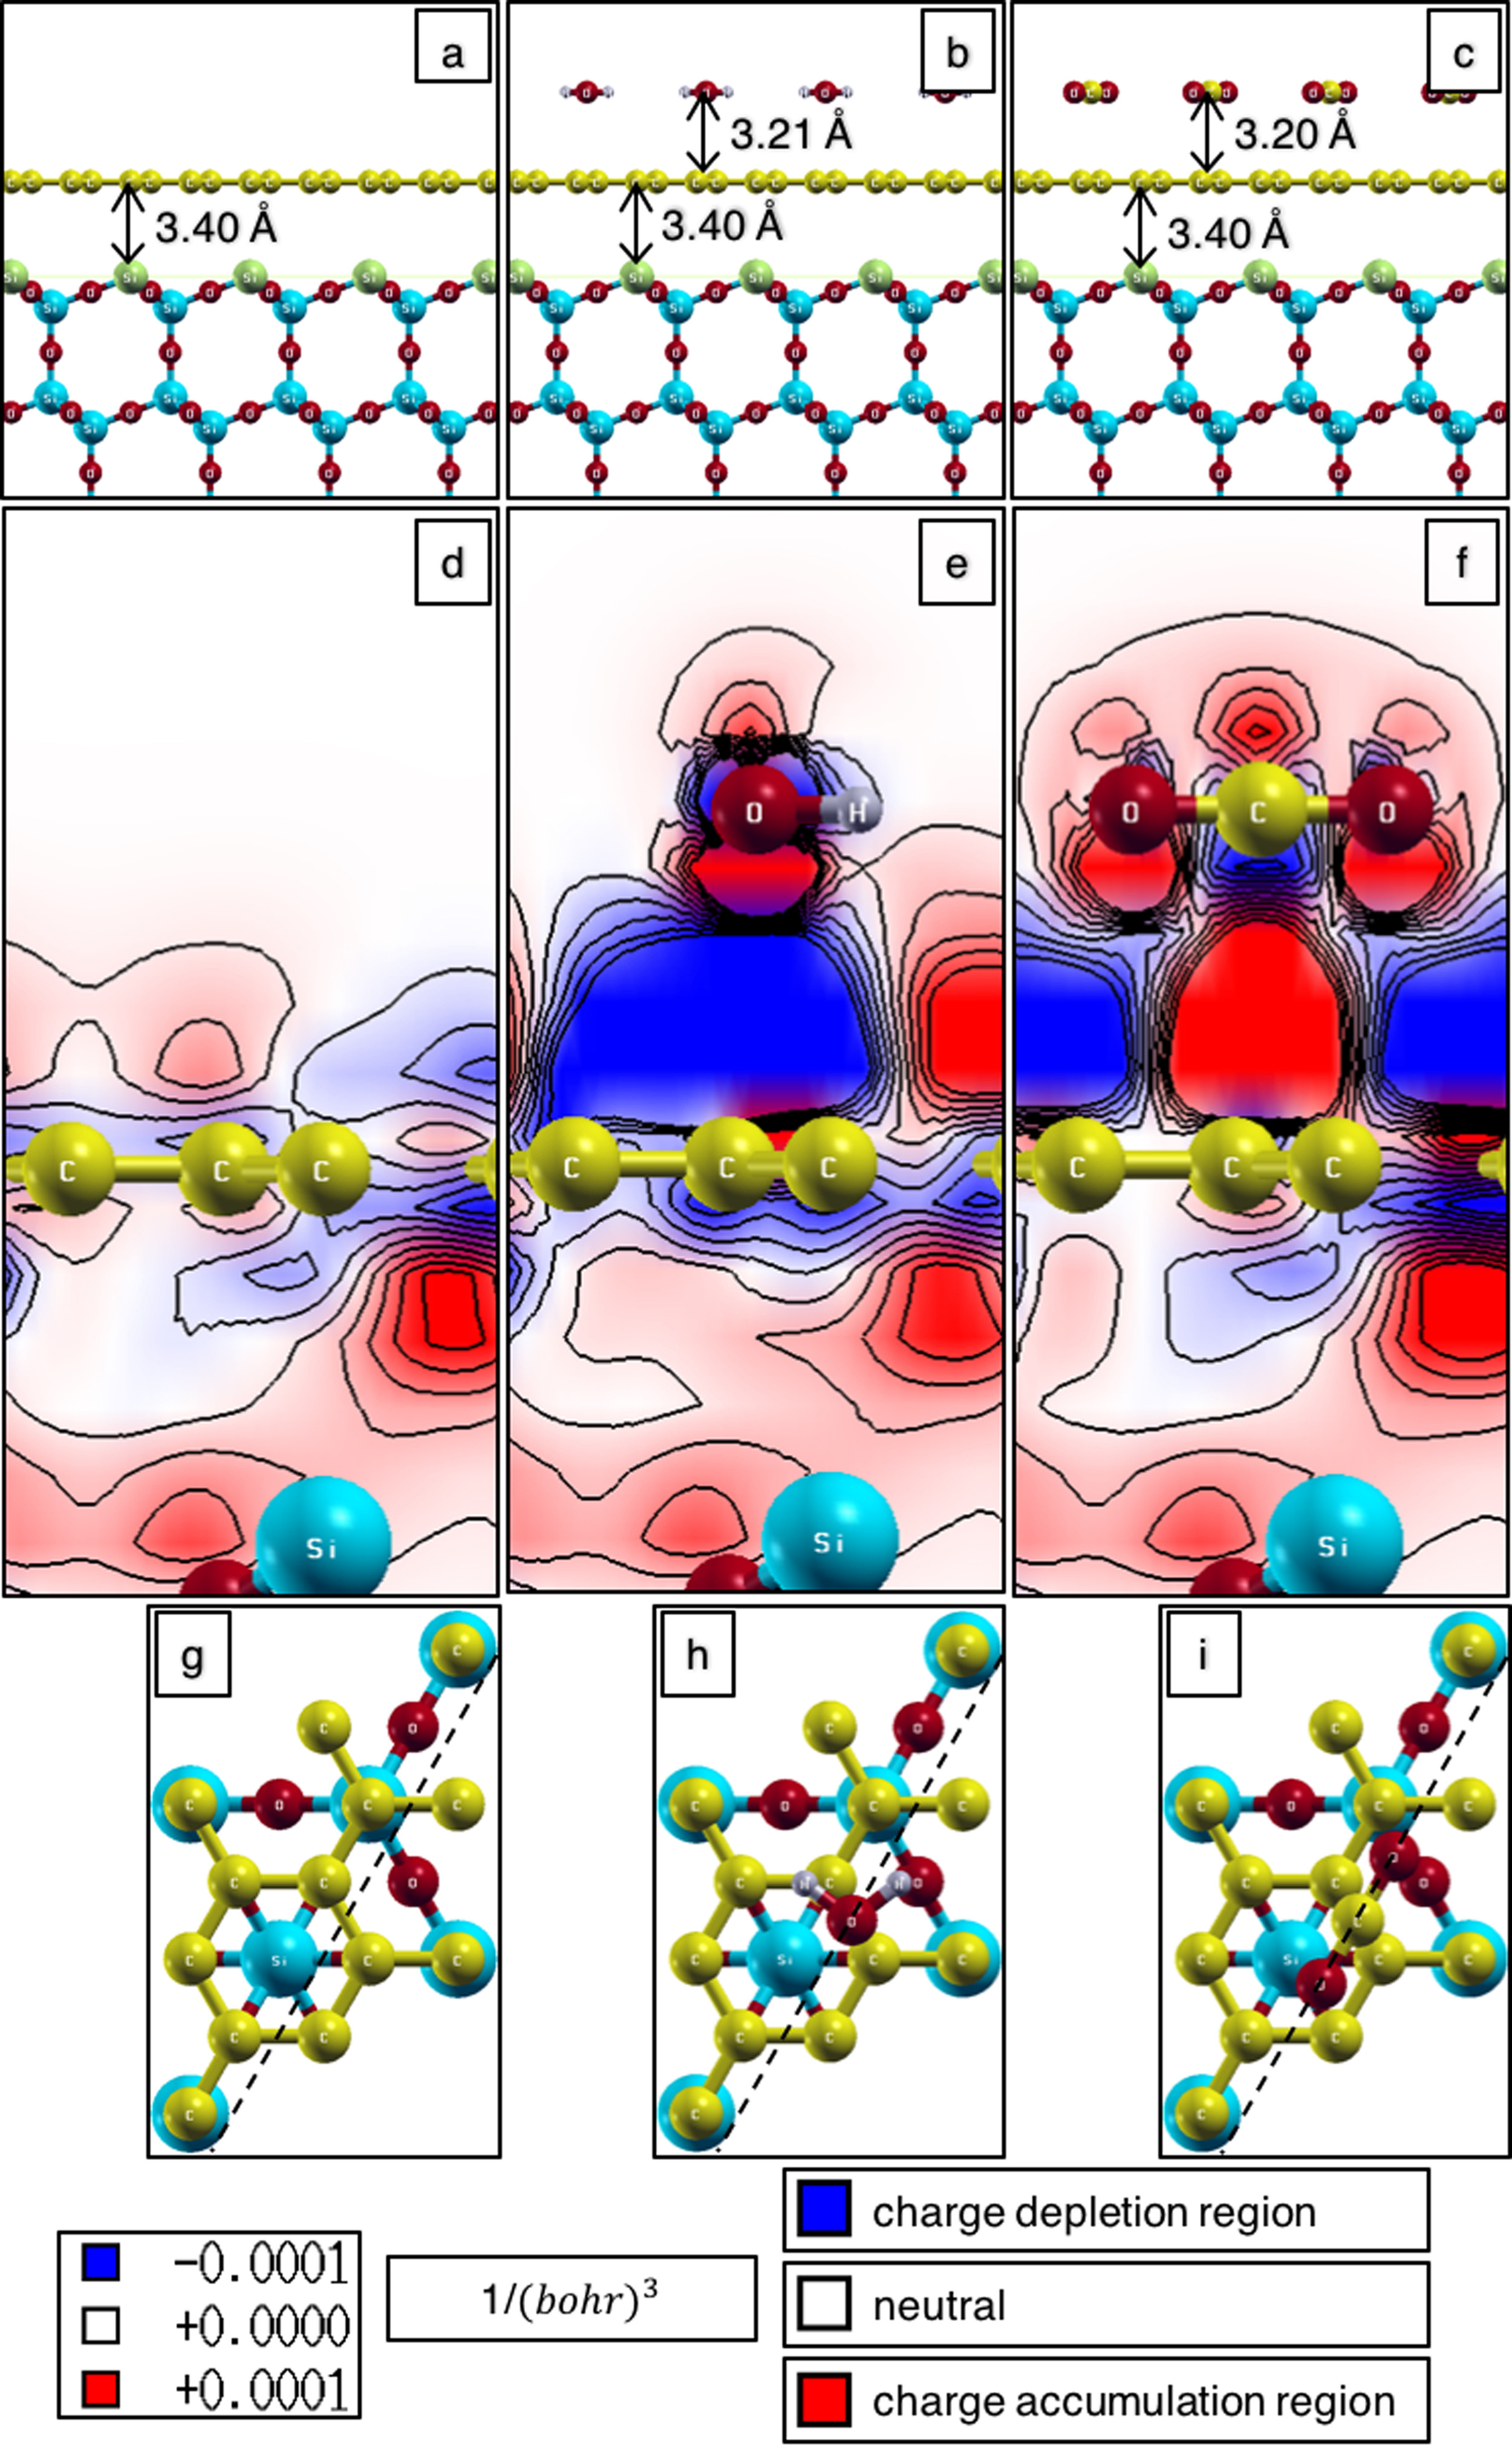
\includegraphics[scale=0.9,keepaspectratio]{Figs/Paper1a.jpg} %[width=\textwidth]
    \caption{excerpt from manuscript describing Paper \hyperref[P1]{$\Rmnum{1}$}~\cite{Elgammal2017}.}
    \label{paper1a}
\end{figure}

Our findings were in line with literature~\cite{Wehling2008}, where the weak interaction between the adsorbate molecules on top of the pristine graphene sheet and the defect states arising from the underlying substrates induces a doping effect in the graphene sheet. That is detailed in Paper \hyperref[P1]{$\Rmnum{1}$}, where the substrate defects effect when combined with water molecules, change the electronic structure properties represented by CDD contours. We studied the substrate defects on three different substrates and found that doping effect took place in all the substrate surface defect types across the three different substrates with different degrees. The substrate slabs were either of silica type ($\beta$-cristobalite and $\alpha$-quartz) or $\alpha$-sapphire. Notably, the defects within the $\beta$-cristobalite substrate surface were the $Q_{\textrm 3}^{\textrm 0}$,  which is a well-known and common silica substrate surface defect~\cite{Wilson2000, Walsh2000}. The defects within the other silica and sapphire substrates type took place at the substrates' surface with either silicon or aluminium undercoordinated atoms terminating the substrates. We referred them to as Si-terminated $\alpha$-quartz (0001) and Al-terminated sapphire (0001) substrates. The respective (CDD) contour plots are available in Fig. \ref{paper1a}, Fig. \ref{paper1b} and Fig. \ref{paper1c} for the three cases respectively.

\begin{figure}
    \centering
    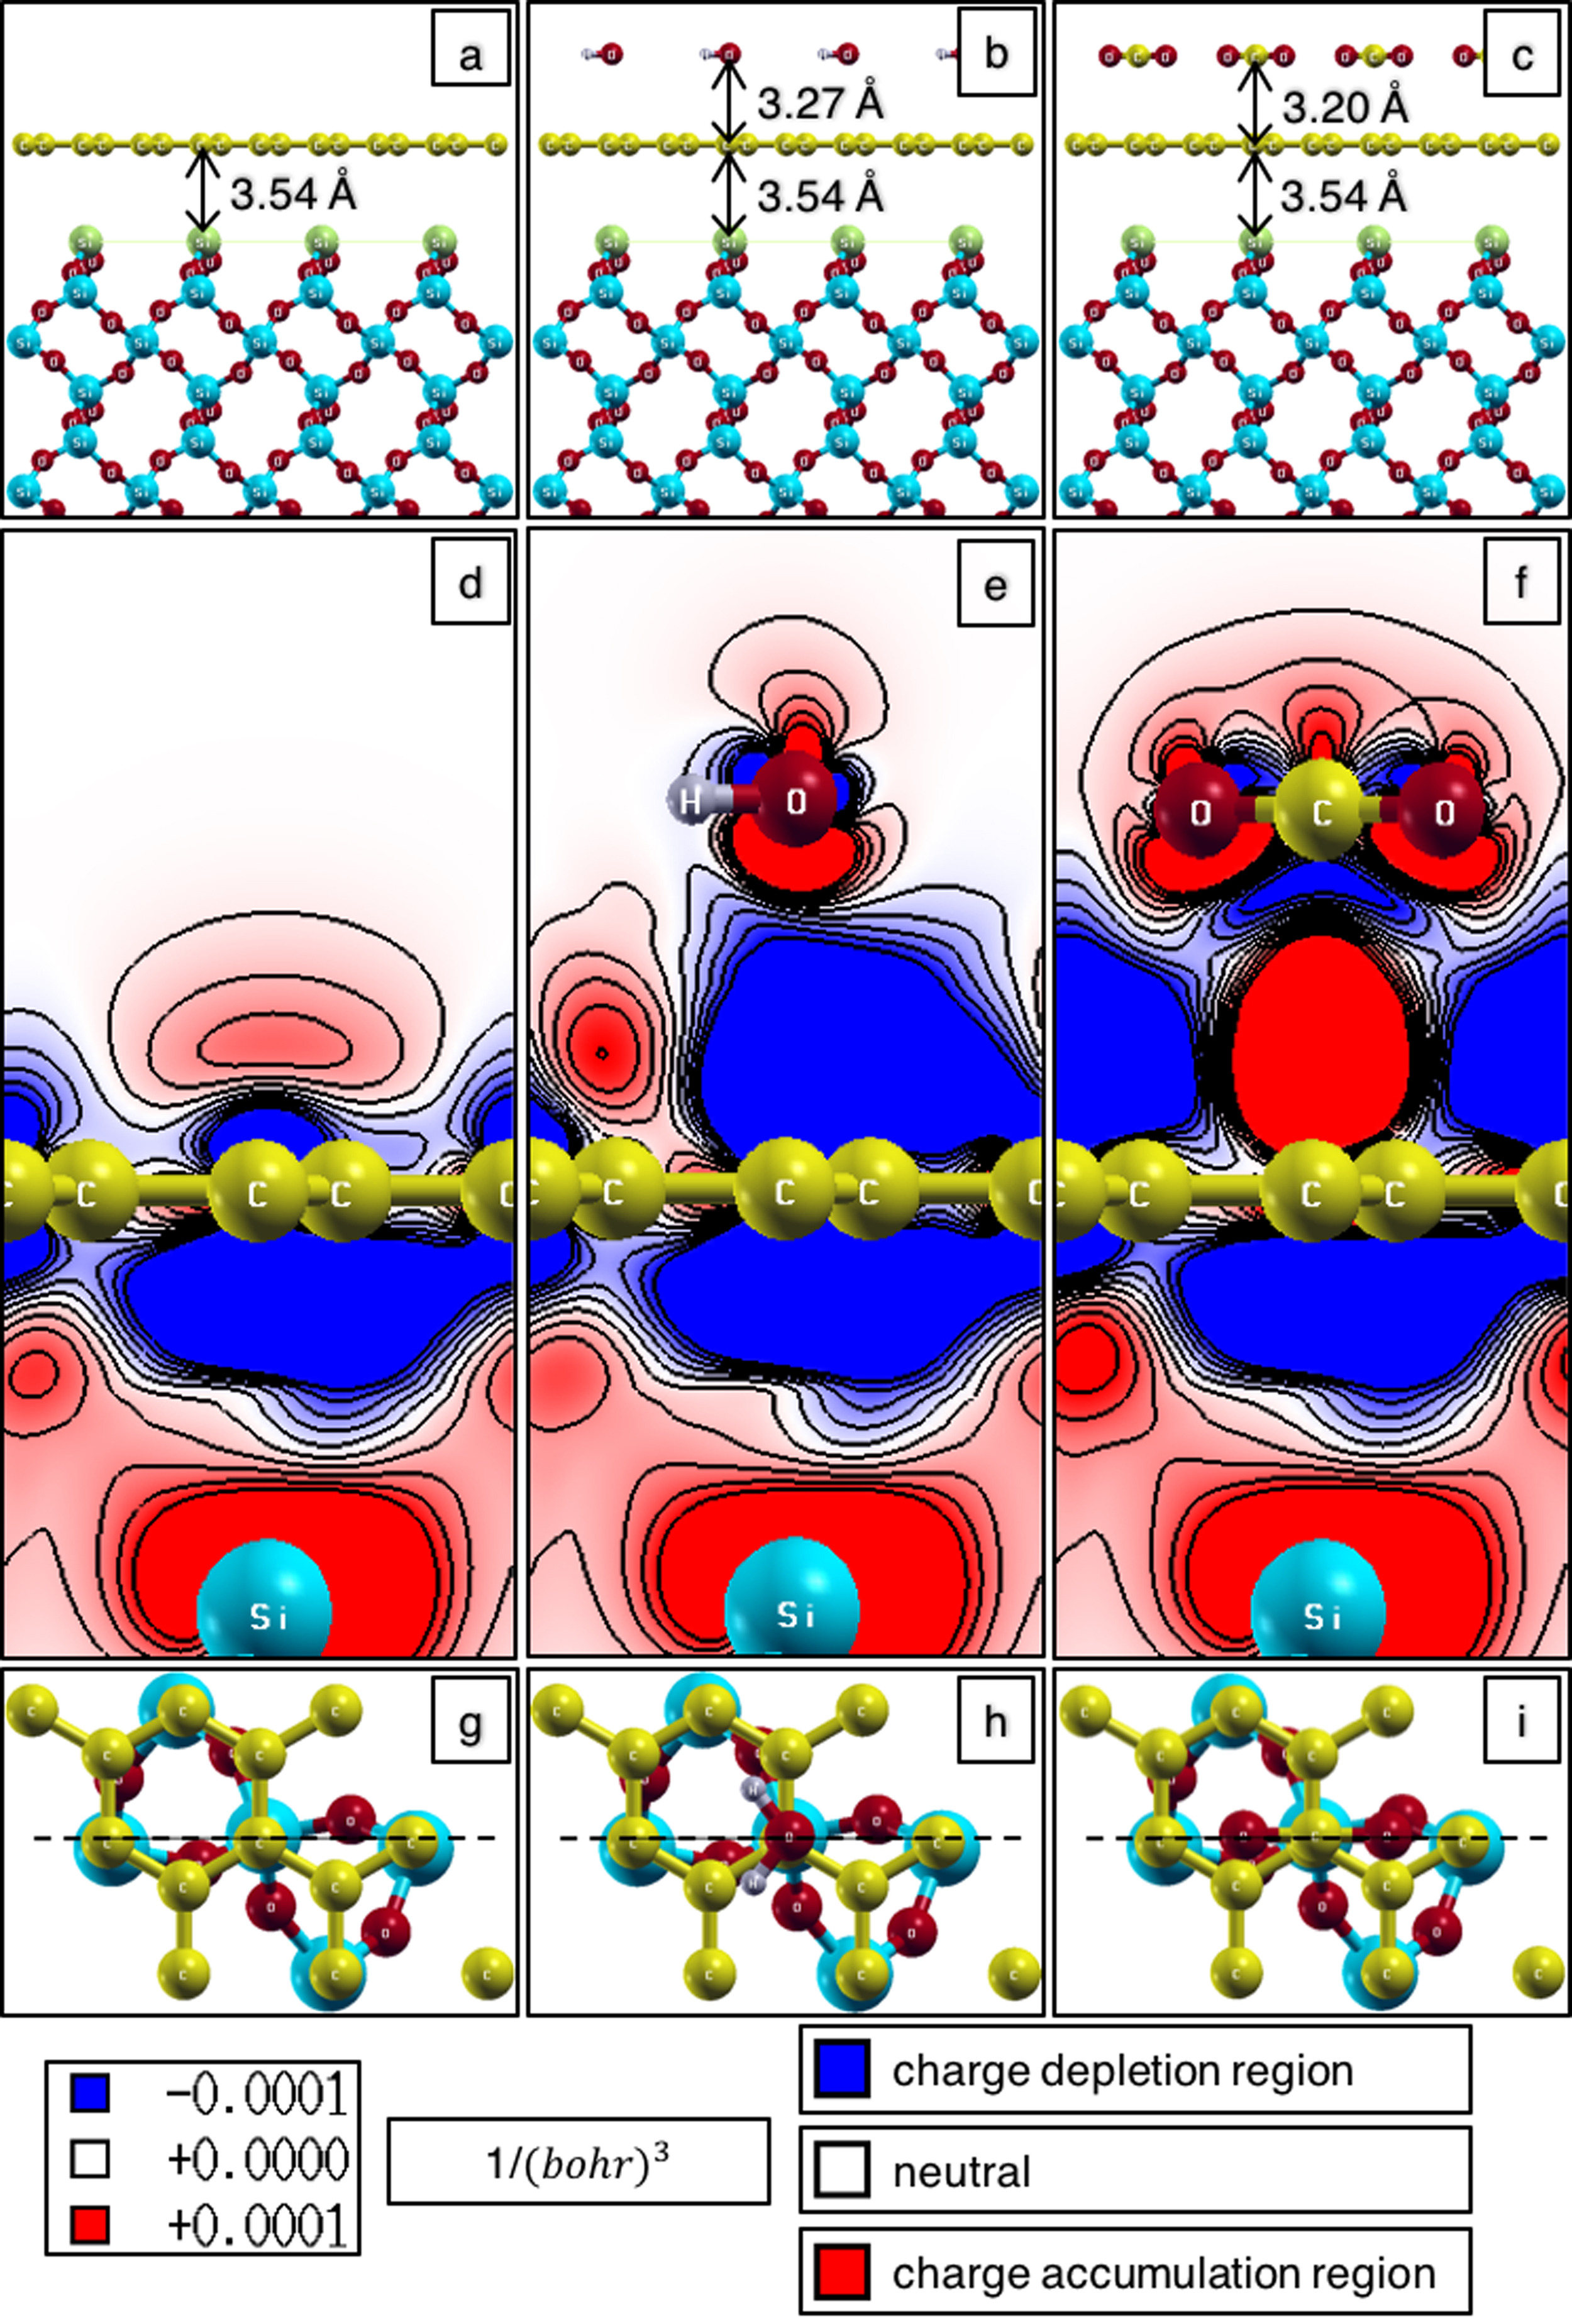
\includegraphics[scale=0.9,keepaspectratio]{Figs/Paper1b.jpg} %[width=\textwidth]
    \caption{excerpt from manuscript describing Paper \hyperref[P1]{$\Rmnum{1}$}~\cite{Elgammal2017}.}
    \label{paper1b}
\end{figure}

\begin{figure}
    \centering
    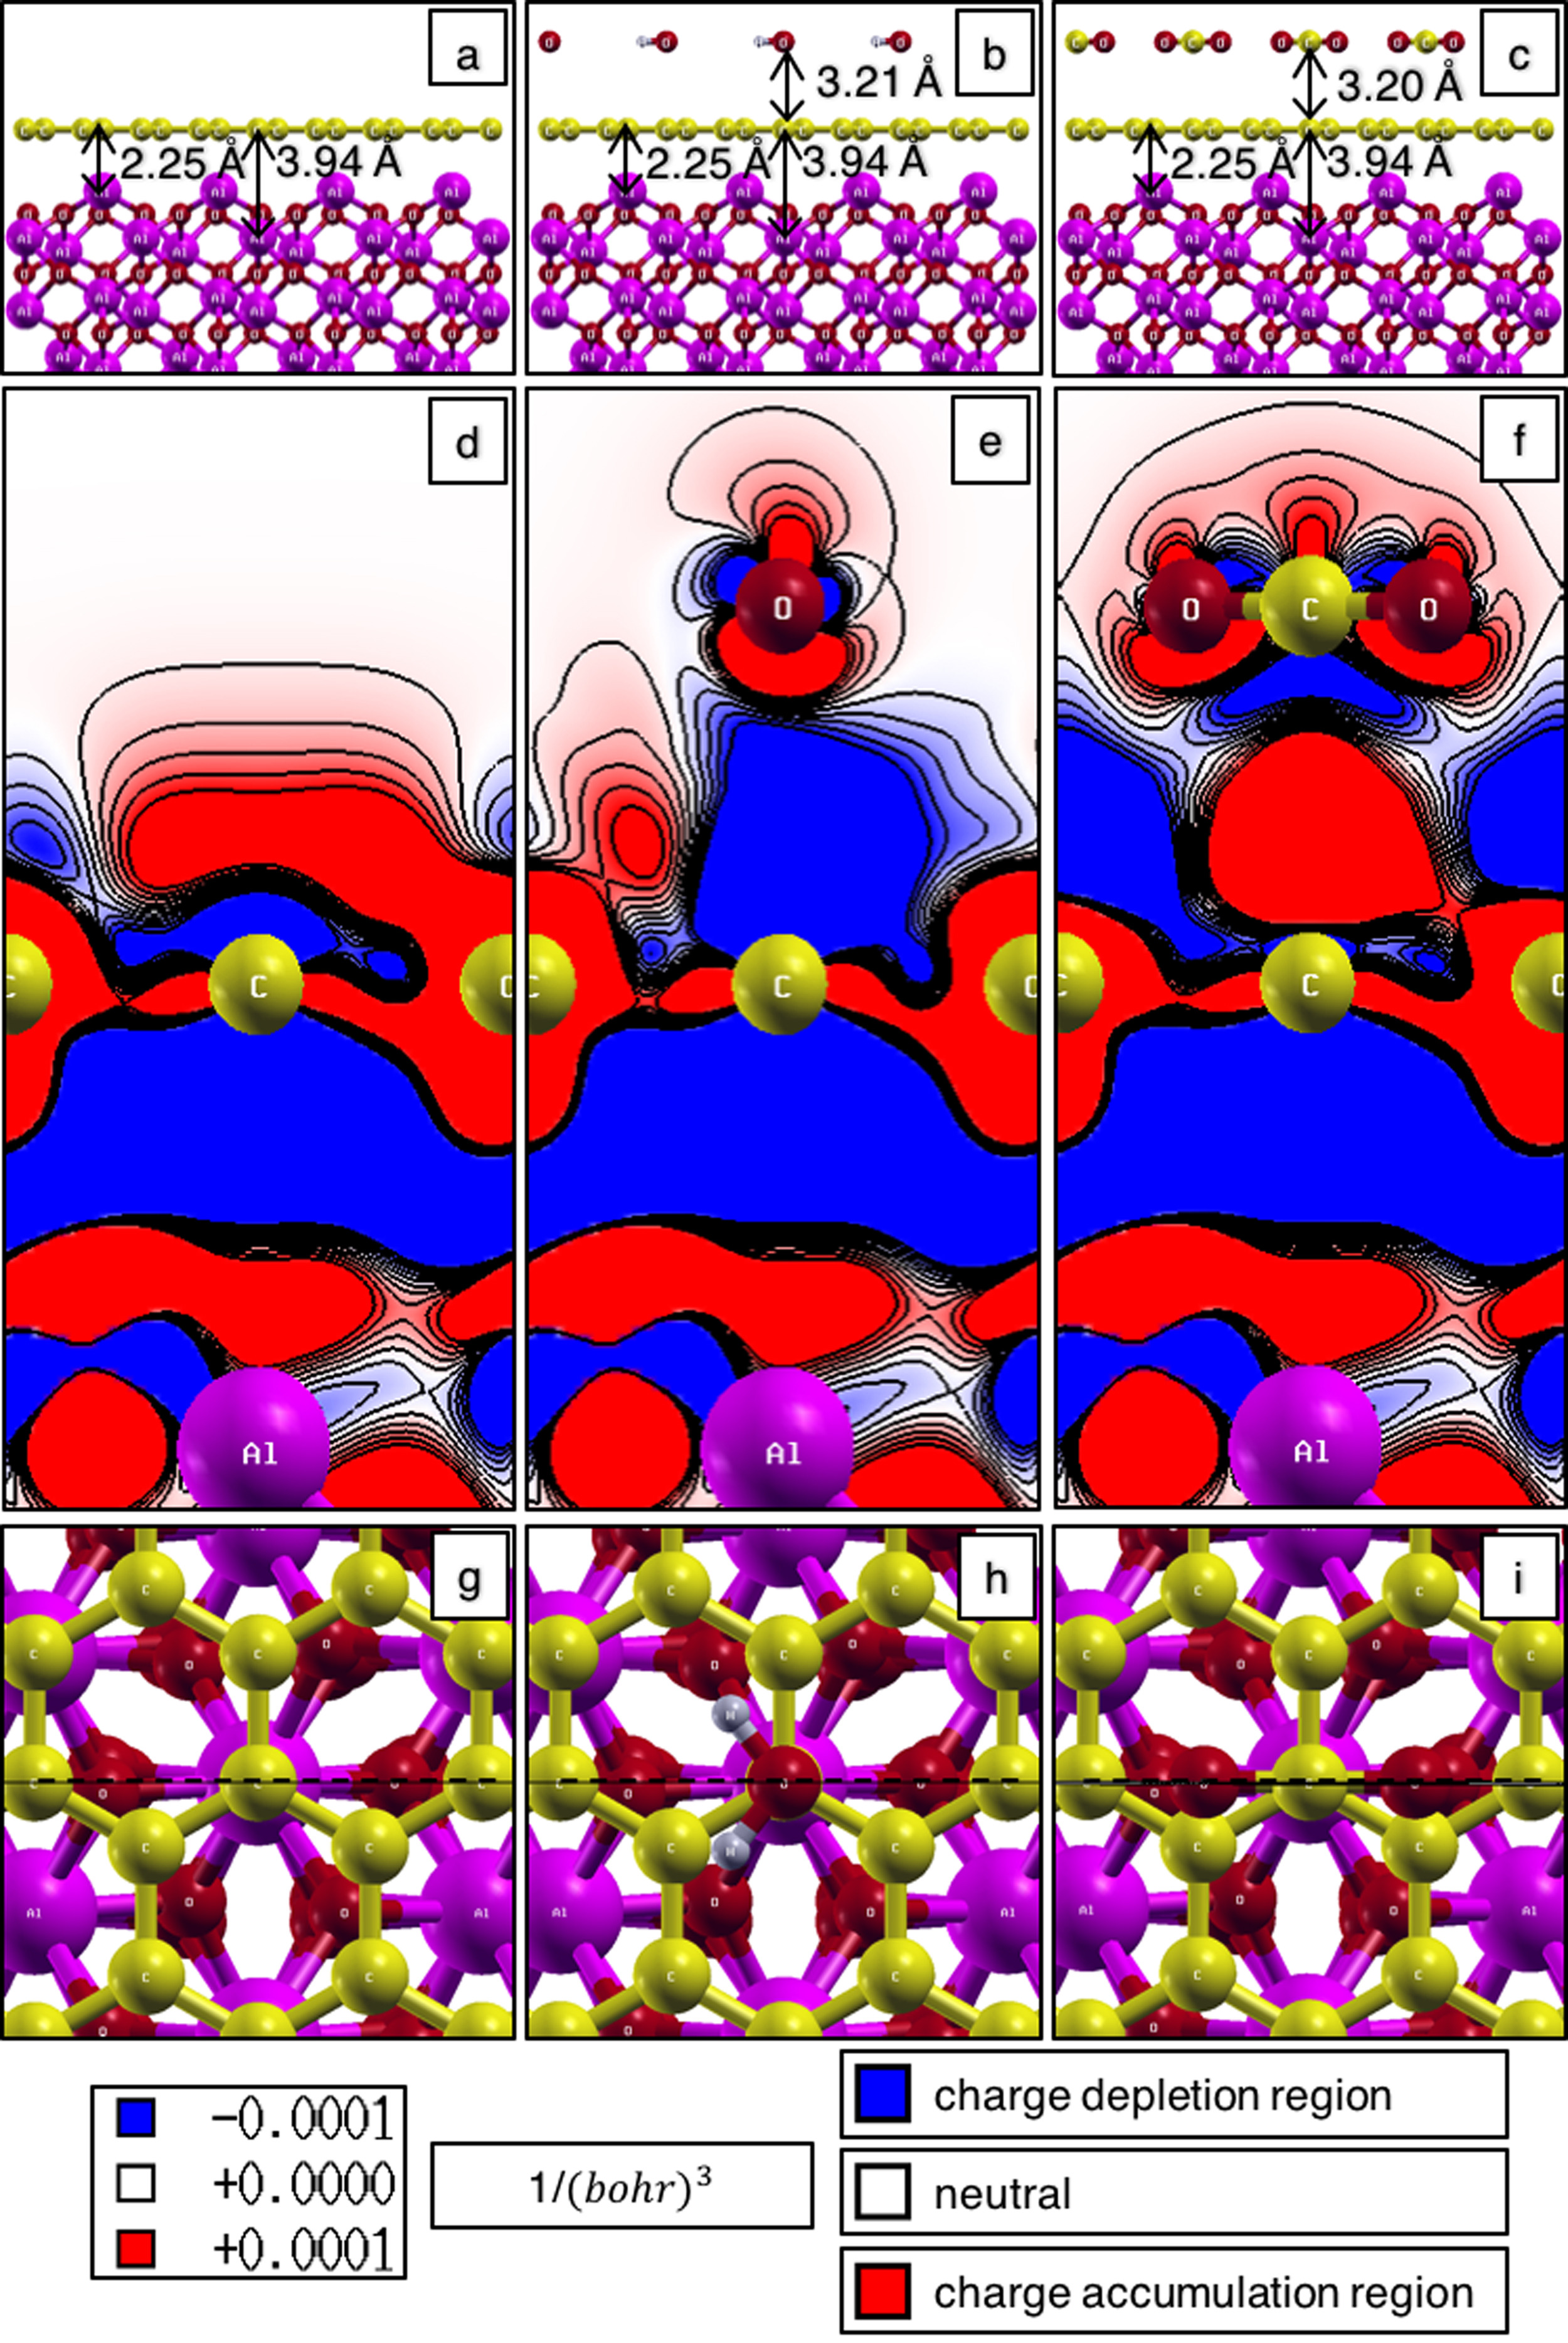
\includegraphics[scale=0.9,keepaspectratio]{Figs/Paper1c.jpg} %[width=\textwidth]
    \caption{excerpt from manuscript describing Paper \hyperref[P1]{$\Rmnum{1}$}~\cite{Elgammal2017}.}
    \label{paper1c}
\end{figure}

In paper \hyperref[P1]{$\Rmnum{1}$}, we examined several adsorbate configurations, distinguished by the relative (x-y) plane positioning of the adsorbates with respect to the graphene sheet. Among all the relaxed configurations, adsorbate configurations with the lowest energy (a preferred configuration) are the closest to the graphene sheet among the same substrate type. This observation is due to a stronger bonding (more hybridisation) that result in a shorter bonding distance. We found that water adsorbates always preferred to be above the centre of the graphene hexagon (hollow sites) regardless of the type of the underlying substrate. Meanwhile, carbon dioxide adsorbates preferred configurations differed according to the substrate. For the cristobalite case: it was on top of the midway between two carbon atoms (the so-called bridge position). For the quartz case: it was on top of silicon atom of the Si-terminated substrate. For the sapphire case: it was on top of a carbon atom in the graphene sheet as well as an aluminium atom (inside the substrate and not the substrate's surface top atom). Moreover, carbon dioxide adsorbates revealed a binding distance of 3.2 Å away from the graphene sheet in all the preferred configurations across all the three cases. We extended this study with paper \hyperref[P2]{$\Rmnum{2}$} taking into consideration a more robust treatment of the dispersion interactions using non-local vdW functionals that we previously discussed in Chapter \ref{DFT-chapter}. As a follow-up, we studied graphene's electronic structure properties being in contact with a different pool of substrate types which can be metal, semiconductor or insulators as in manuscript \hyperref[P3]{$\Rmnum{3}$}. Moreover, we found good agreement with experimental equilibrium distances and binding energies (or adhesive energies).
\clearpage
In summary, upon studying those different systems, we can conclude that, with the presence of the adsorbates, the doping effect differs slightly per different types of adsorbates within the silica substrates, while it differs dramatically in comparison with sapphire substrate type. Sapphire can be embedded as a coating material silicon substrates~\cite{Jadaun2011}. Thus, we can conclude that the effect of adsorbates existence on the graphene sheet can depend heavily on the substrate properties, types and its associated defects as previously reported in~\cite{Wehling2008}.

\begin{figure}
    \centering
    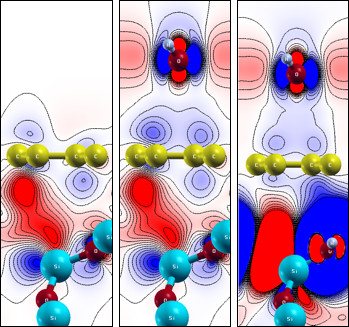
\includegraphics[width=\textwidth]{Figs/Paper4.png}
    \caption{excerpt reprinted from manuscript describing Paper \hyperref[P4]{$\Rmnum{4}$}~\cite{Smith2015}.}
    \label{paper4}
\end{figure}

In Papers \hyperref[P4]{$\Rmnum{4}$}, \hyperref[P5]{$\Rmnum{5}$}, we studied similar systems to the ones in Papers \hyperref[P1]{$\Rmnum{1}$}, \hyperref[P2]{$\Rmnum{2}$} in conjunction with experimental input. We showed in both articles a qualitative overview on the influence of substrate-surface defects on pristine graphene sheet with either water or carbon dioxide molecules adsorbed on top. The results showed a difference in the charge distribution when comparing cases lacking adsorbates with cases of adsorbates existence as shown per Figs. (\ref{paper4}), (\ref{paper5}). Besides, there is a difference in the CDD contours according to the surface conditioning, as we examined cases of hydrogen-passivated and non-passivated surface termination as shown in Fig. (\ref{paper4}). The CDD contours experience alternating charge depletion and accumulation regions throughout the graphene sheet depending on the different ambient condition it can coexist according to the examined cases.

\begin{figure}
    \centering
    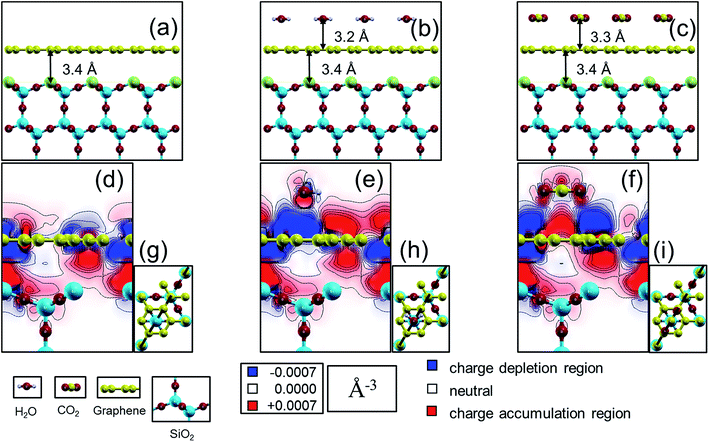
\includegraphics[width=\textwidth]{Figs/Paper5.png} %[scale=0.5,keepaspectratio]
    \caption{excerpt from manuscript describing Paper \hyperref[P5]{$\Rmnum{5}$}~\cite{Smith2017}.}
    \label{paper5}
\end{figure}

We expanded the study to double layered graphene, which has caught interesting properties leading to useful utilisation in sensor devices~\cite{Melios2016, Yakovkin2016}. We performed a related joint-experimental study in~\cite{Xuge2017} via DFT calculations on pristine double layered graphene residing on one type of $\alpha$-quartz substrate. The CDD contour plots depicted in Fig. (\ref{paper6}) revealed that the double-layered graphene isolates the combined doping effect of the substrate and the adsorbates, that we already discussed before. Each layer is concerned with the adhered weakly-bounded system which are the substrate and the adsorbates. Furthermore, the overall charge transfer was also small, signalling value of 0.05e and 0.04e as a net charge transfer towards the adsorbate molecules of carbon dioxide and water molecules.

\begin{figure}
    \centering
    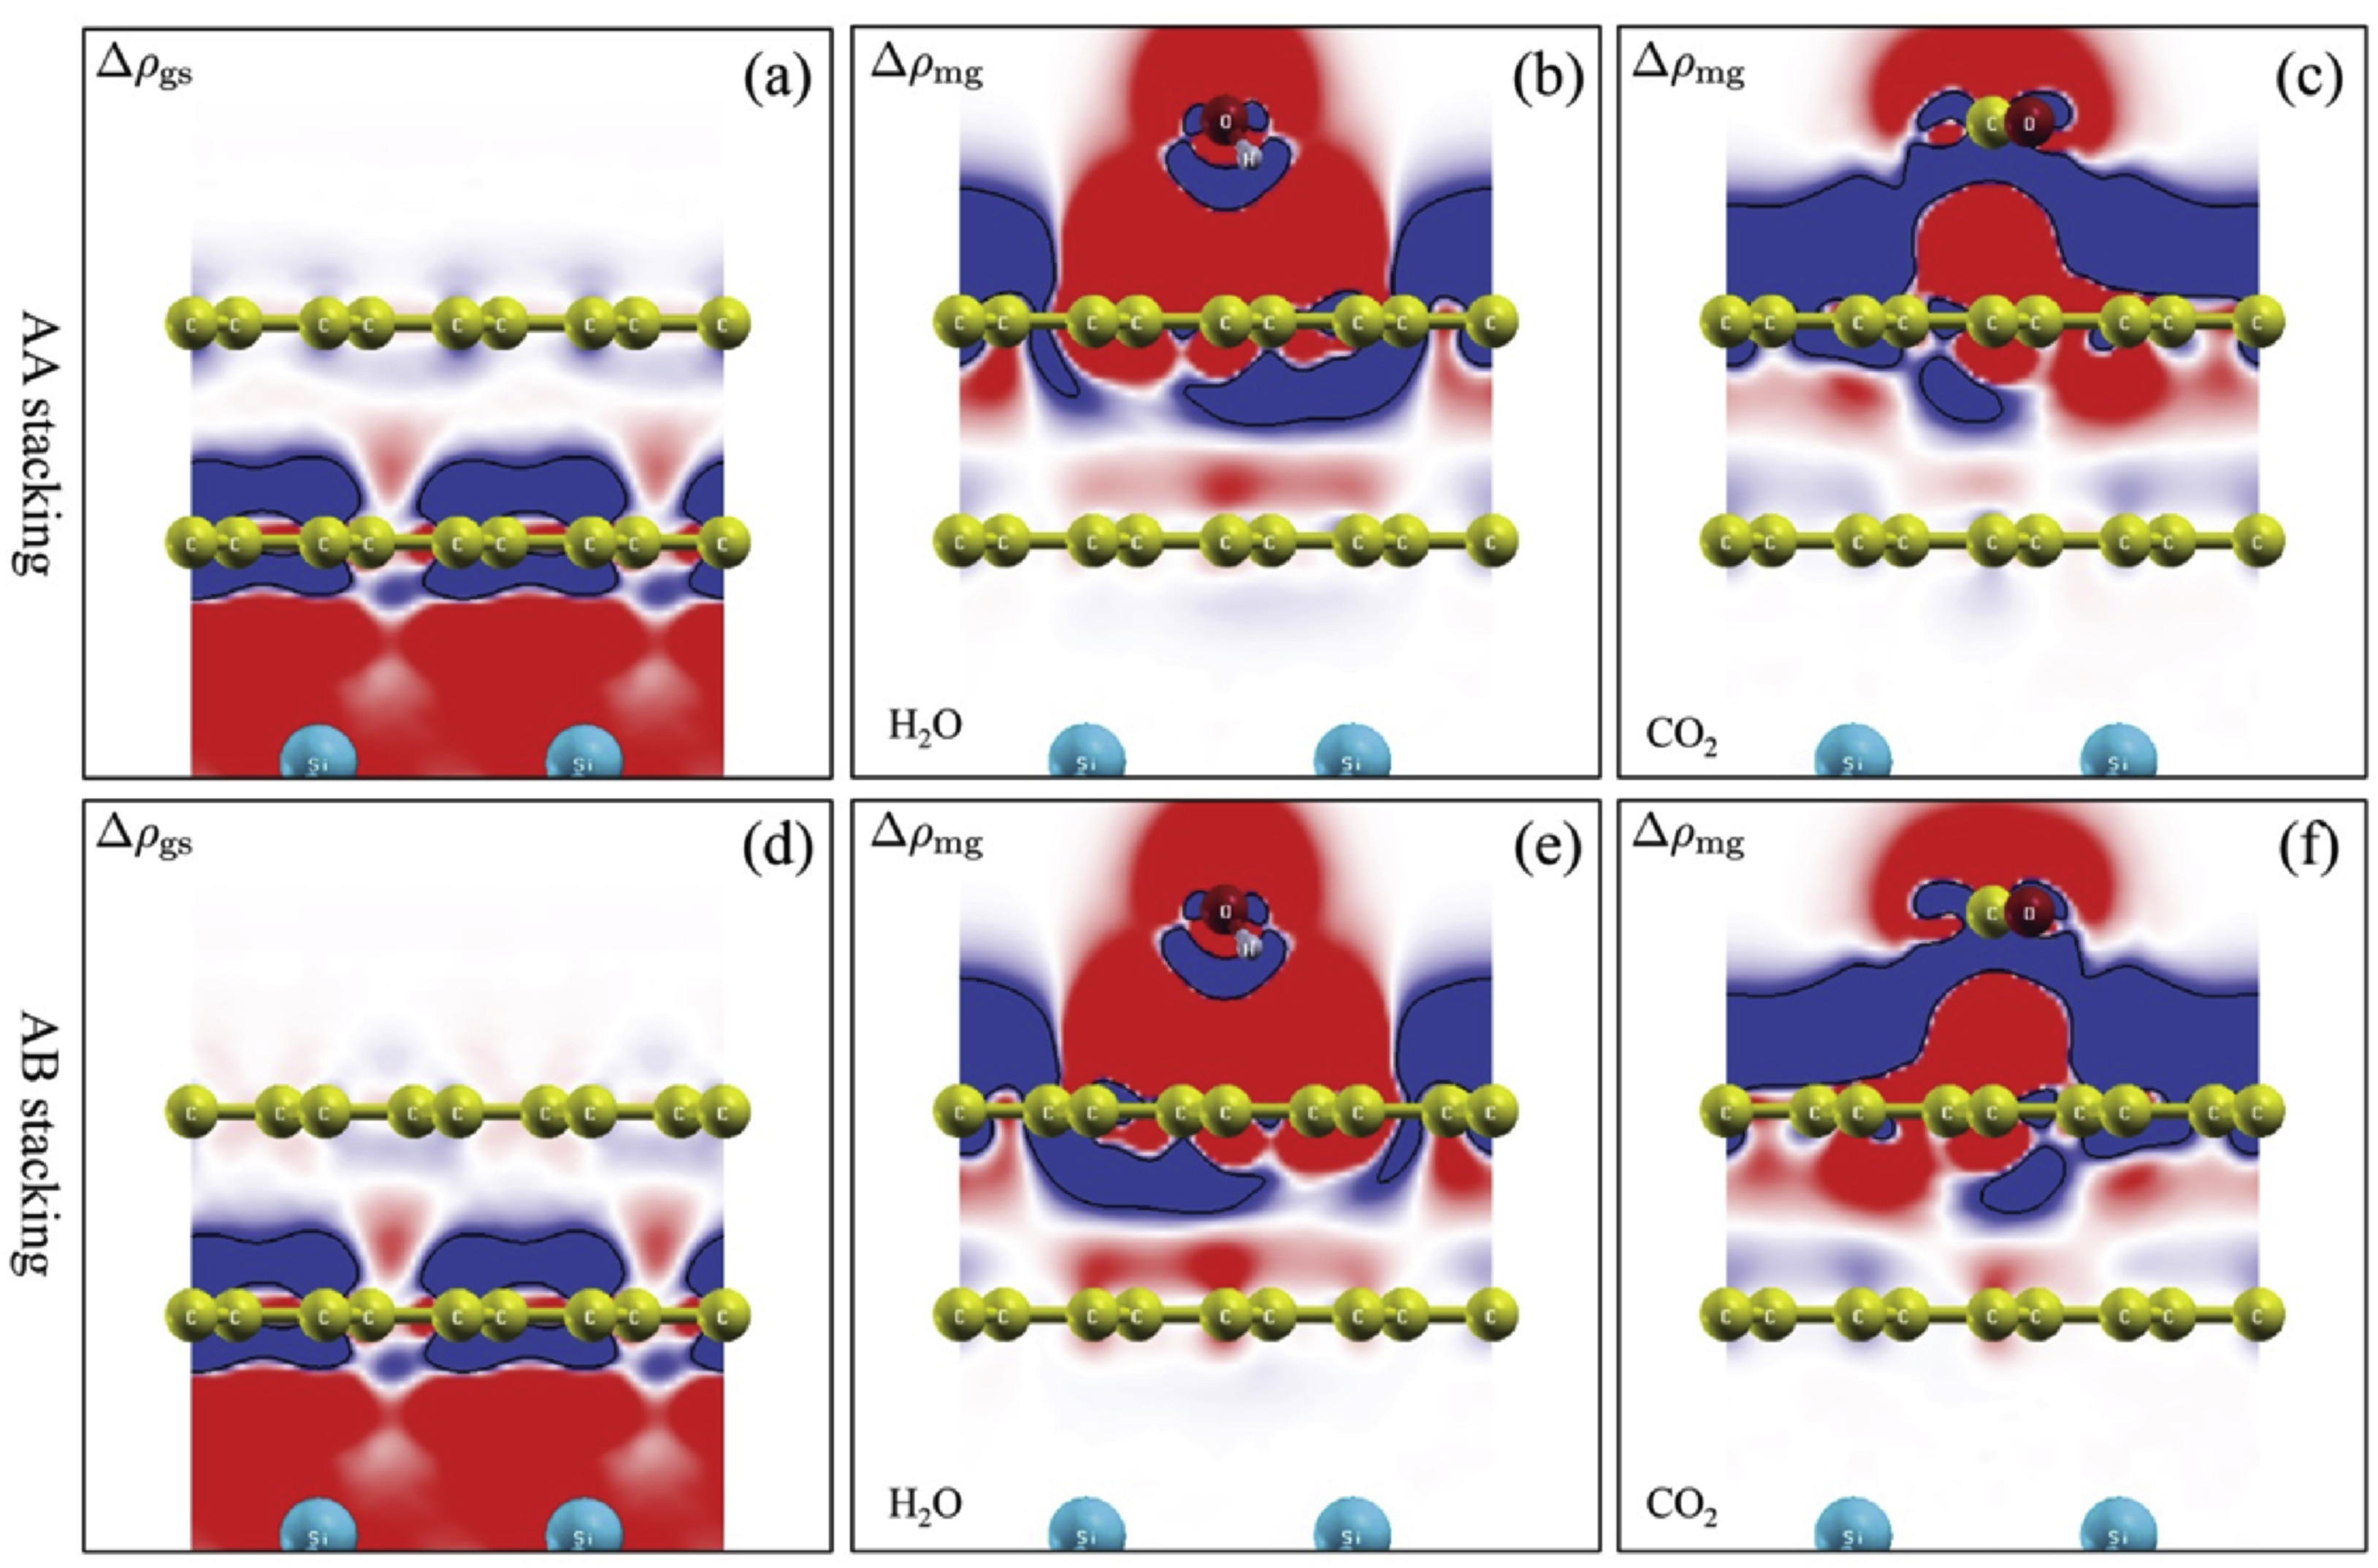
\includegraphics[width=\textwidth]{Figs/Paper6.jpg} %[scale=0.8,keepaspectratio]    
    \caption{excerpt from manuscript describing Paper \hyperref[P6]{$\Rmnum{6}$}~\cite{Xuge2017}.}
    \label{paper6}
\end{figure}

As the ultimate goal of designing such devices is to obtain higher value systems according to the \textit{more than Moore} paradigm we pointed to in Chapter \ref{introduction}, we need to isolate different components and functionalities on the same chip in order not to interfere with each-other and comply with the targeted diversification purpose. Thus, we performed a combined experimental and theoretical study as in~\cite{Smith2016} for confirming the passivating layers effect on the graphene-based sensors and how the associated CDDs looks like as rendered in Fig. \ref{paper7}. We showed with an availability of a passivation layer in between the graphene and adsorbates that the adsorbates effect on the graphene sheet is dysfunctioned.

\begin{figure}
    \centering
    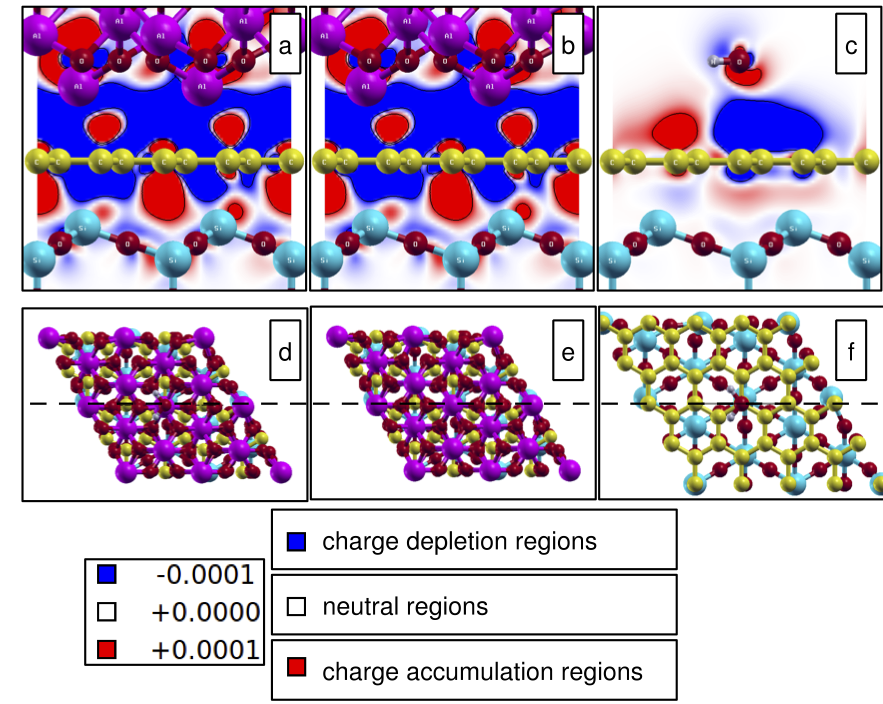
\includegraphics[width=\textwidth]{Figs/Paper7.png}
    \caption{excerpt from manuscript describing Paper \hyperref[P7]{$\Rmnum{7}$}~\cite{Smith2016}\textcopyright 2016 IEEE.}
    \label{paper7}
\end{figure}
\endinput